\chapter{Vereinheitlichung zweier Messungen des \protect\boldmath\texorpdfstring {$t\bar{t}\gamma$}{math}-Produktionswirkungsquerschnitts mit dem EFT\textit{fitter}}%
In diesem Kapitel erfolgt die Kombination der Messungen von ATLAS und CMS für den $t\bar{t}\gamma$-Produktionswirkungsquerschnitt bei einer Schwerpunktsenergie von $\sqrt{s} = \SI{8}{\tera\electronvolt}$. Da die Messungen in unterschiedlichen Phasenräumen erfolgt sind, wird vor der eigentlichen Kombination mit dem EFT\textit{fitter} eine Phasenraumstudie durchgeführt, um die Phasenräume zu vereinheitlichen.

\section{\texorpdfstring {$t\bar{t}\gamma$}{math}-Messungen von ATLAS und CMS}%
\label{kap:messung}
Die Messungen des Produktionswirkungsquerschnitts von ATLAS und CMS sind beide in Proton-Proton-Kollisionen bei einer Schwerpunktsernegie von $\sqrt{s}=\SI{8}{\tera\electronvolt}$ durchgeführt worden. Die Bestimmung des Wirkungsquerschnitts erfolgt über einen Endzustand mit Lepton und Jets. Somit zerfällt eins der entstehenden $W$-Bosonen in ein Elektron oder Myon mit dem entsprechenden Neutrino und das andere $W$-Boson hadronisch. Ein möglicher Feynman-Graph für diesen Prozess ist in~\ref{fig:tta} dargestellt.\\
Obwohl ATLAS und CMS den gleichen Prozess betrachtet haben, unterscheiden sich die Messungen grundlegend durch den zu Grunde liegenden Phasenraum, im folgenden mit \textit{fiducial} (fid) bezeichnet. Die Wahl den \textit{fiducial} Phasenraum für die EFT-Interpretation zu betrachten, hat den Vorteil, dass die Extrapolation in den experimentell nicht messbaren Phasenraum minimiert wird, wodurch die Modellunabhängigkeit maximiert wird. Die von ATLAS und CMS verwendeten Schnitte für den \textit{fiducial} Phasenraum sind in Tabelle \ref{tab:cut}
aufgeführt.\\
%
 \begin{table}[H]
     \centering
    \begin{tabular}{c|l|l}
      Objekte & ATLAS & CMS \\
      \hline
      \textbf{Photon} & $p_T > \SI{15}{\giga\electronvolt}\quad |\eta| < 2,37$ & $p_T > \SI{25}{\giga\electronvolt}\quad |\eta| < 1,44$\\
      Leptonen & $p_T > \SI{25}{\giga\electronvolt}\quad |\eta| < 2,5$ & $\text{e}:\: p_T > \SI{35}{\giga\electronvolt}\quad |\eta| < 2,5$ \\
      {} & {} & $\symup{\mu}:\: p_T > \SI{26}{\giga\electronvolt}\quad |\eta| < 2,5$\\
      Jets & $p_T > \SI{25}{\giga\electronvolt}\quad |\eta| < 2,5$ & $p_T > \SI{30}{\giga\electronvolt}\quad |\eta| < 2,4$\\
      b-Jets & $p_T > \SI{5}{\giga\electronvolt}$ &  \\
      $E^{miss}_T$ &  & $p_T^{miss} > \SI{20}{\giga\electronvolt}$
    \end{tabular}
    \caption{Verwendete Schnitte auf den \textit{fiducial} Phasenraum.}
    \label{tab:cut}
 \end{table}
Dabei fällt auf, dass sich die Schnitte für das Photon deutlich unterscheiden. So setzt ATLAS einen Transversalimpuls von $p_{T} > \SI{15}{\giga\electronvolt}$ voraus, wohingegen CMS mindestens $p_{T} > \SI{25}{\giga\electronvolt}$ einfordert. Außerdem wählt ATLAS eine Pseudorapidität von $|\eta| < 2,37$, während CMS $|\eta| < 1,44$ annimmt. Zudem setzt CMS einen fehlenden Transversalimpuls von $p_{T}^{miss} > \SI{20}{\giga\electronvolt}$ voraus.
ATLAS setzt zudem zwischen dem Photon und dem Lepton mindestens einen Abstand von $\symup{\Delta} R(\gamma, \ell) = 0,7$, zwischen dem Photon und dem Jet $\symup{\Delta} R(\gamma, \text{Jet}) = 0,5$ und zwischen dem $b$-Quark und dem Jet $\symup{\Delta} R(\text{b}, \text{Jet}) = 0,3$ vorraus.
Das CMS-Papier umfasst keine weiteren Angaben zur Isolation der Objekte.\\
Die von ATLAS und CMS gemessenen Produktionswirkungsquerschnitte für $t\bar{t}\gamma$ ergeben sich zu:
\begin{align*}
  \sigma^{fid, \text{ATLAS}}_{t\bar{t}\gamma} &= 139 \pm 18~\text{(stat.$+$syst.)}~ \si{\femto\barn}\\
  \sigma^{fid, \text{CMS}}_{t\bar{t}\gamma, e} &= 138 \pm 45~\text{(stat.$+$syst.)}~ \si{\femto\barn}\\
  \sigma^{fid, \text{CMS}}_{t\bar{t}\gamma, \mu} &= 115 \pm 32~\text{(stat.$+$syst.)}~ \si{\femto\barn}.
\end{align*}
CMS unterscheidet dabei zwischen Wirkungsquerschnitten, bei denen das Lepton im Endzustand einmal ein Elektron und einmal ein Myon ist.

\section{Kombination mit dem EFT\textit{fitter}}
Der EFT\textit{fitter}~\cite{Castro:2016jjv} ist ein Programm, das es ermöglicht Studien zur BSM-Physik auf Grundlage von effektiven Feldtheorien durchzuführen. Er erlaubt Benutzern physikalische Modelle selbst zu implementieren und im Rahmen Bayes'scher Statistik zu testen. Zudem ist eine Kombination verschiedener Messungen möglich. Bei solchen Kombinationen ist die Breite Wahrscheinlichkeitsverteilung für den kombinierten Wert der Messergebnisse und damit ihre Aussagekraft von der Anzahl der Messungen abhängig.
Die Bayessche Inferenz ermöglicht eine Anpassung des Modells an die Daten, sodass eine Wahrscheinlichkeitsverteilung für den gesuchten Parameter des Modells erhalten wird.\\
Die Grundlage für diese Berechnungen liefert der Satz von Bayes:
\begin{align}
  p(\lambda|\vec{x}) = \frac{L(\vec{x}|\lambda) \cdot \pi(\lambda)}{p(\vec{x})}.
\end{align}
Der gesuchte Parameter des Modells ist $\lambda$ und die verwendete Datenmenge wird in diesem Fall durch $\vec{x}$ beschrieben. Die A-Prioriverteilung $\pi(\lambda)$ enthält Informationen über die zu untersuchende Variable $\lambda$.
Die Normierung $p(\vec{x})$ wird mit:
\begin{align}
  p(\vec{x}) = \int d\lambda L(\vec{x}|\lambda) \cdot \pi(\lambda)
\end{align}
berechnet. Die Likelihood $L(\vec{x}|\lambda)$ beschreibt die Wahrscheinlichkeitsverteilung der Daten $\vec{x}$. Die gesuchte Posteriorverteilung wird durch $p(\lambda|\vec{x})$ beschrieben. Diese beinhaltet neue Erkenntnisse über den Parameter $\lambda$, die aus den Daten gewonnen werden. Somit kann die anfängliche Erkenntnis über den Parameter $\lambda$ verbessert werden.\\
Werden für eine Kombination $n$ Messungen $x_i$ mit $(i= 1,...,n)$ und $N$ Observablen $y_i$ mit $(i= 1,...,N)$ betrachtet und kann die Likelihood als gaußförmig angenommen werden, kann sie durch:
\begin{align}
  -2 \ln{L(\vec{x}|\lambda)} = \sum^{n}_{i=1} \sum^{n}_{j=1} \left[\vec{x} - U\vec{y}\right]_{i} \mathcal{M}_{ij}^{-1} \left[\vec{x} - U\vec{y}\right]_{j}
  \label{eqn:like}
\end{align}
beschrieben werden. $U_{ij}$ ist das Matrixelement einer $n \times N$-Matrix $U$, welches eins ist, wenn $x_i$ die Messung zur Observable $y_i$ ist und ansonsten Null. Da die Unsicherheiten der Messung $x_i$ korreliert sein können, beschreibt
\begin{align}
  \mathcal{M}_{ij} = \text{cov}[x_i, x_j] = \sum_{k=1}^{M} \text{cov}^{(k)}[x_i, x_j]
\end{align}
die Elemente der symmetrischen und positiv semidefiniten Kovarianzmatrix, bei der $M$ die Anzahl der verschiedenen Quellen an Unsicherheiten ist. Der EFT\textit{fitter} basiert auf der BLUE-Methode (\textit{best linear unbiased estimator})~\cite{LYONS1988110}, deshalb werden für Kombinationen die gleichen Ergebnisse erhalten.

\section{Phasenraumstudie mit MadGraph5}
\label{phasencms}
Um eine Kombination der beiden Messungen des $t\bar{t}\gamma$-Wirkungsquerschnitts von CMS und ATLAS ermöglichen zu können, muss zuvor eine Phasenraumstudie durchgeführt werden. Da beide Messungen in unterschiedlichen Phasenräumen durchgeführt wurden, müssen sie zunächst vereinheitlicht werden. Die Vergrößerung eines Phasenraums erfolgt als erste Approximation durch einen Faktor, der zwischen den beiden Phasenräumen liegt. Dazu können mit Hilfe des Monte-Carlo-Generators MadGraph5~\cite{Alwall:2014hca} (MG) zunächst die beiden Produktionswirkungsquerschnitte für $t\bar{t}\gamma$ berechnet werden.
Anschließend werden diese beiden Werte durcheinander geteilt und der sich ergebende Faktor wird auf die CMS-Messung angewandt. Dadurch wird diese Messung in den Phasenraum der ATLAS-Messung extrapoliert.\\
Zunächst einmal wird der Lepton+Jet-Zerfall des $t\bar{t}$-Quarkpaars unter Abstrahlung des Photons mit den expliziten Endzuständen in MG simuliert.
Dazu wird das SM als Modell und der $\text{CTEQ}6\text{L}1$ PDF-Satz~\cite{Paakkinen:2018zbs} zum Implementieren des Prozesses genutzt. Bei der Berechnung des Lepton+Jet-Endzustands wird nur die führende Ordnung (\textit{leading-order}, LO) betrachtet. Für die Berechnung der Produktionswirkungsquerschnitte werden die in Kapitel~\ref{kap:messung} angegebenen Schnitte genutzt.
Da von der CMS-Kollaboration in dem Papier keine weiteren Aussagen über die Isolation der einzelnen Objekte gemacht werden, werden für diese Arbeit die gleichen Abstände wie bei ATLAS verwendet.
Unter diesen Vorraussetzungen ergeben sich die Wirkungsquerschnitte aus der MG Simulation zu:
\begin{align}
  \sigma^{fid, \text{ATLAS}}_{\text{LO}} &= 146,5 \pm 0,095~ \si{\femto\barn}\\
  \sigma^{fid, \text{CMS}}_{\text{LO}} &= 49,29 \pm 0,034~ \si{\femto\barn}.
\end{align}
Auffällig ist dabei, dass der Wert von ATLAS $2,97$ mal so groß ist, wie der von CMS gemessene Produktionswirkungsquerschnitt. Dies ist unerwartet, da beide Ergebnisse der Messungen sehr ähnlich sind und in den Papieren als vertäglich mit dem SM angesehen werden.
Beim Vegleich der Photon-Schnitte fällt jedoch auf, dass durch den höheren $p_T$-Schnitt von CMS bereits ungefähr $90000$ der anfänglichen $220000$ Ereignisse verloren gehen. Durch den Schnitt auf die Pseudorapidität entfallen ebenfalls nochmal etwa $45000$ Ereignisse. Dies entspricht etwa $\SI{60}{\percent}$ der anfänglichen Ereignisse, sodass der Faktor $3$ durchaus plausibel erscheint. Eine Veranschaulichung dieser Änderungen befindet sich in Abbildung~\ref{fig:schnitte}.\\
\begin{figure}
    \begin{subfigure}[c]{0.5\textwidth}
      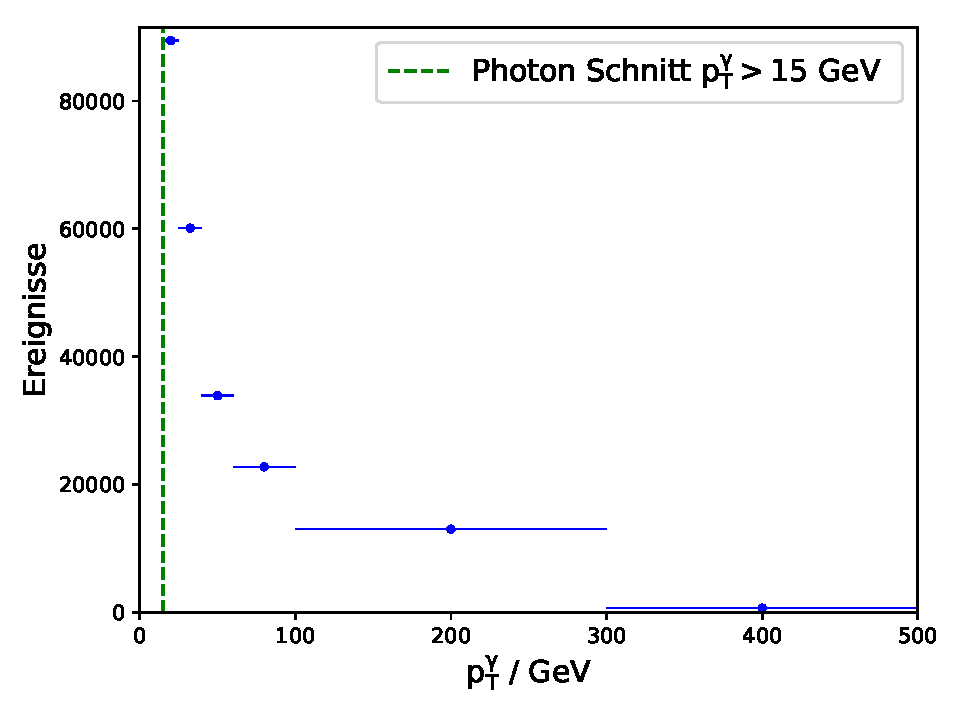
\includegraphics[width=\textwidth]{Plots/photon_pt_Atlas.pdf}
      \subcaption{ATLAS}
    \end{subfigure}
    \begin{subfigure}[c]{0.5\textwidth}
      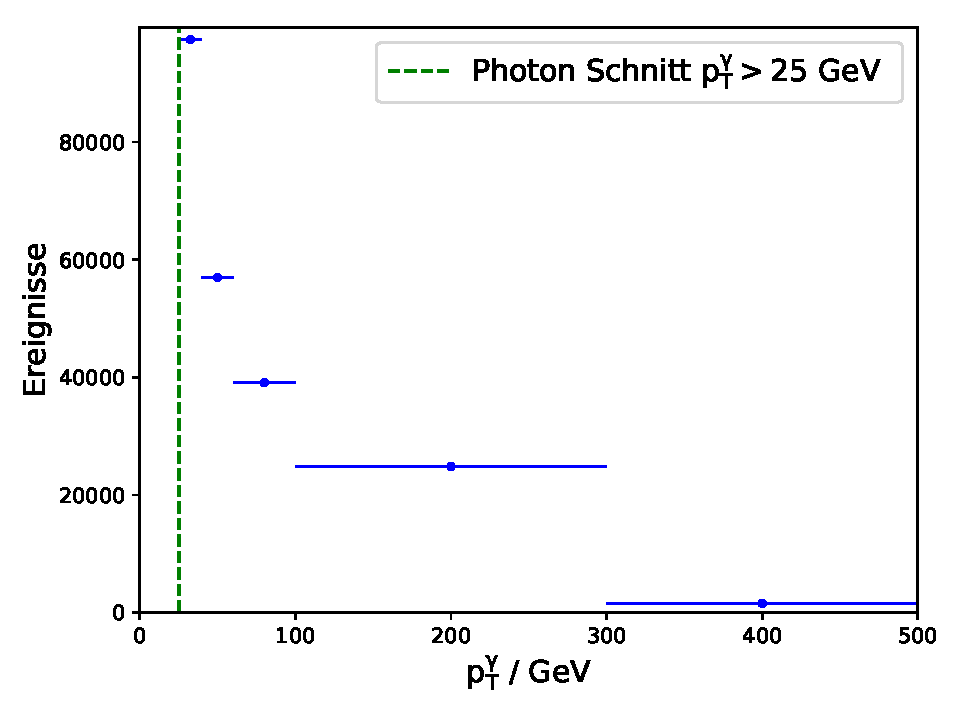
\includegraphics[width=\textwidth]{Plots/photon_pt_Cms.pdf}
      \subcaption{CMS}
    \end{subfigure}
    \begin{subfigure}[c]{0.5\textwidth}
      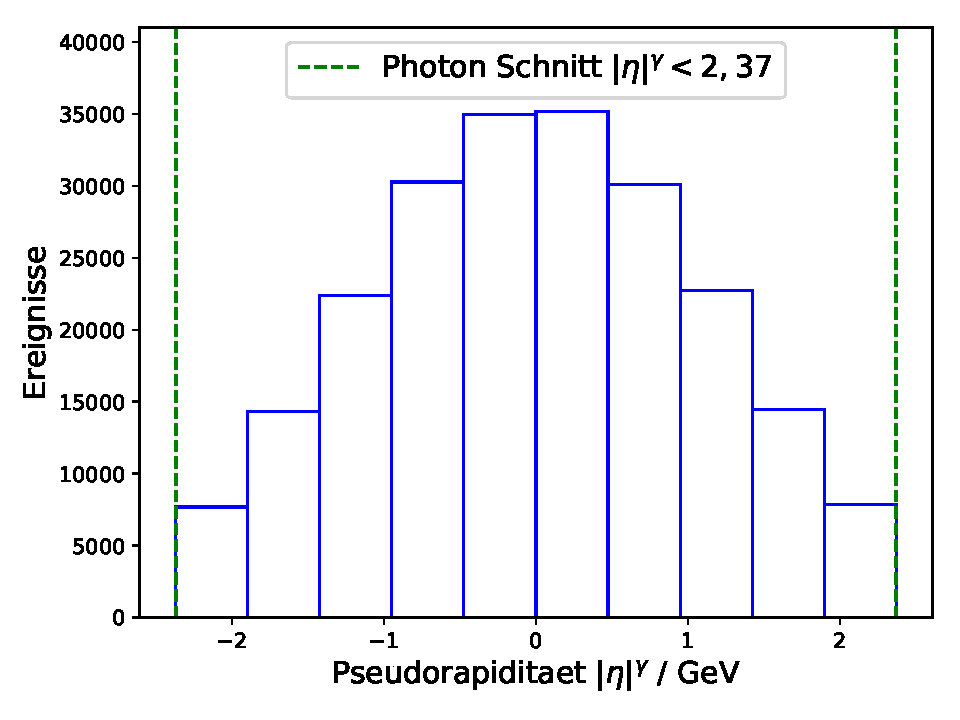
\includegraphics[width=\textwidth]{Plots/photon_eta_Atlas.pdf}
      \subcaption{ATLAS}
    \end{subfigure}
    \begin{subfigure}[c]{0.5\textwidth}
      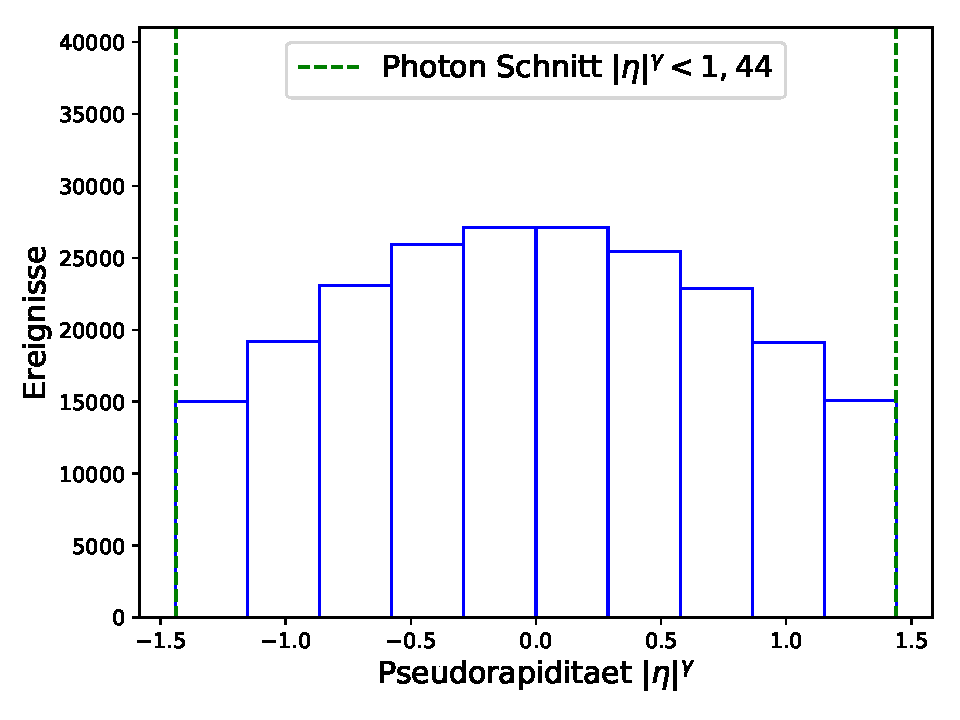
\includegraphics[width=\textwidth]{Plots/photon_eta_Cms.pdf}
      \subcaption{CMS}
    \end{subfigure}
    \caption{Verteilungen der Transversalimpulse und der Pseudorapidität der Photonen. Die grünen Linien representieren die von ATLAS und CMS verwendeten Schnitte des \textit{fiducial} Phasenraums. Die verwendeten Datensätze stammen aus Simulationen dieser Schnitte mit MadGraph5.}
    \label{fig:schnitte}
\end{figure}
Um einen möglichst genauen Faktor zwischen den \textit{fiducial} Phasenräumen zu erhalten, wird eine Rechnung in der nächst-führenden Ordnung (\textit{next-to-leading-oder}, NLO) angestrebt. Dafür wird in MG der Prozess $p~p~$\textrightarrow$~t~\bar{t}~\gamma$~, ohne expliziten Endzustand, sowohl in LO als auch in NLO, simuliert. Daraus kann im Anschluss ein $k$-Faktor als Näherung zwischen den beiden Ordnungen berechnet werden.\\
Für die Berechnung werden sowohl die Faktorisierungsskala $\mu_{F}$ als auch eine Renomierungsskala $\mu_{R}$ dynamisch gewählt.
Damit ergeben sich folgende Wirkungsquerschnitte in der LO-Rechnung:
\begin{align}
  \sigma^{\text{ATLAS}}_{\text{LO}} &= 682,8 \pm 3,9~ \si{\femto\barn}\\
  \sigma^{\text{CMS}}_{\text{LO}} &= 361,6 \pm 1,5~ \si{\femto\barn}
\end{align}
und folgende Werte in der NLO-Rechnung:
\begin{align}
  \sigma^{\text{ATLAS}}_{\text{NLO}} &= 452,5 \pm 1,2~ \si{\femto\barn}\\
  \sigma^{\text{CMS}}_{\text{NLO}} &= 243,6 \pm 0,7~ \si{\femto\barn}.
\end{align}
Da diese Wirkungsquerschnitte keine Abstrahlung von Zerfallsprodukten beinhalten, lassen sie sich durch Multiplizieren mit dem Verzweigungsverhältnis (\textit{branching ratio}, $\mathrm{BR}$) für den Lepton+Jets-Zerfall in die expliziten Endzustände umrechnen.
Das Verzweigungsverhältnis gibt die Wahrscheinlichkeit an, dass ein Zustand in einen bestimmten Endzustand zerfällt und liegt in diesem Fall bei $\mathrm{BR}\approx\SI{30}{\percent}$. Werden die Wirkungsquerschnitte nun mit dem $\mathrm{BR}$ multipliziert und der NLO-Wert durch den der LO-Rechnung geteilt, ergibt sich folgender $k$-Faktor für ATLAS und CMS:
\begin{align}
  k_{\text{ATLAS}} &= \frac{0,3 \cdot 682,8~ \si{\femto\barn}}{0,3 \cdot 452,5~ \si{\femto\barn}} = 1,509 \pm 0,010\\
  k_{\text{CMS}} &= \frac{0,3 \cdot 361,6~ \si{\femto\barn}}{0,3 \cdot 243,6~ \si{\femto\barn}} = 1,484 \pm 0,008.
\end{align}
Unter Anwendung dieser $k$-Faktoren auf die zu Beginn bestimmten Produktionswirkungsquerschnitte ergibt sich der Phasenraumfaktor $f$ zwischen den \textit{fiducial} Phasenräumen von ATLAS und CMS zu:
\begin{align}
  f = \frac{1,509 \cdot 146,5~ \si{\femto\barn}}{1,484 \cdot 49,29~ \si{\femto\barn}} = 3,0221 \pm 0,0028.
\end{align}
Es ergibt sich erneut ein Faktor, der nahe an drei liegt. Somit wird der CMS-Phasenraum durch Multiplizieren mit einem Phasenraumfaktor von ungefähr drei in den von ATLAS transformiert. Dabei ergeben sich die folgenden Produktionswirkungsquerschnitte für die modifizierten gemessenen CMS-Wirkungsquerschnitte:
\begin{align}
  \sigma^{fid(A), \text{CMS}}_{t\bar{t}\gamma, e} &= 410 \pm 140~ \si{\femto\barn}\\
  \sigma^{fid(A), \text{CMS}}_{t\bar{t}\gamma, \mu} &= 350 \pm 100~ \si{\femto\barn}.
\end{align}
Problematisch ist, dass bei dieser Rechnung auch die Unsicherheiten extrapoliert werden. Jedoch sind diese nur im \textit{fiducial} CMS-Phasenraum gültig. Diese Umrechnung wird trotzdem gewählt, da es sich lediglich um eine erste Näherung für die Vereinheitlichung der beiden Referenzphasenräume handelt. Dies bedarf weitergehender Studien durch eine aufwändigere Betrachtung der Unsicherheiten.
%
%
\chapter{Kombination der \texorpdfstring {$t\bar{t}\gamma$}{math}-Messungen}
In diesem Kapitel wird die Kombination der ATLAS- und CMS-Messungen unter der Verwendung des Ergebnisses aus Kapitel~\ref{phasencms} beschrieben. Hierbei ist zu beachten, dass die Kombination zuerst unter der Annahme erfolgt, dass zwischen den drei Messergebnissen keine Korrelationen vorliegen. Um diese Annahme zu rechtfertigen, wird anschließend eine Korrelationsstudie für die Korrelation zwischen den beiden CMS-Messungen durchgeführt. Zudem wird der Einfluss einer Korrelation zwischen ATLAS und CMS untersucht.

\section{Kombination}
\label{kombi}
Wird eine Kombination des angegebenen Produktionswirkungsquerschnitts von ATLAS und der in den \textit{fiducial} Phasenraum von ATLAS erweiterten Messungen von CMS mit dem EFT\textit{fitter} unter der Annahme durchgeführt, dass die Messungen nicht korreliert sind, ergibt sich der Wirkungsquerschnitt des Prozesses $p~p \rightarrow~t\bar{t}\gamma$ zu:
\begin{align}
  \sigma_{\text{Kombi}} = 150 \pm 18~ \si{\femto\barn}.
\end{align}
Auffällig ist, dass das kombinierte Ergebnis sehr dicht an dem von ATLAS gemessenen Wert liegt.
Dies ist damit zu begründen, dass eine Gewichtung der gegebenen Messungen anhand ihrer Unsicherheiten durchgeführt wird.
Durch die Extrapolation der Unsicherheiten der CMS-Messungen liegen diese in der selben Größenordnung wie die Nominalwerte von ATLAS, sodass diese Wirkungsquerschnitte bei der Berechnung der Kombination nur sehr gering beitragen.
Bei der Betrachtung der gaußförmigen Verteilungen um den gemessenen Produktionswirkungsquerschnitt in Abbildung~\ref{fig:gau} fällt auf, dass die Verteilungen der CMS-Messungen auf Grund der großen Unsicherheiten deutlich breiter sind und somit die ATLAS-Messung genauer ist.
Dies erklärt die geringe Gewichtung der CMS-Messungen durch den EFT\textit{fitter}.\\
Dieses Ergebnis zeigt neben den Ergebnissen aus Kapitel~\ref{phasencms}, dass eine Kombination zweier Messungen nur zu einem Informationsgewinn führt, wenn sich die Messungen im selben beziehungsweise annährend identischen Phasenraum befinden. Zudem bietet es sich an, eine Korrelationsstudie durchzuführen, um zu überprüfen, ob eine angenommene Korrelation Auswirkungen auf das Ergebnis der Kombination hat und somit die Annahme unkorrelierter Messungen in der Kombination überhaupt gerechtfertigt ist.

\begin{figure}
  \centering
  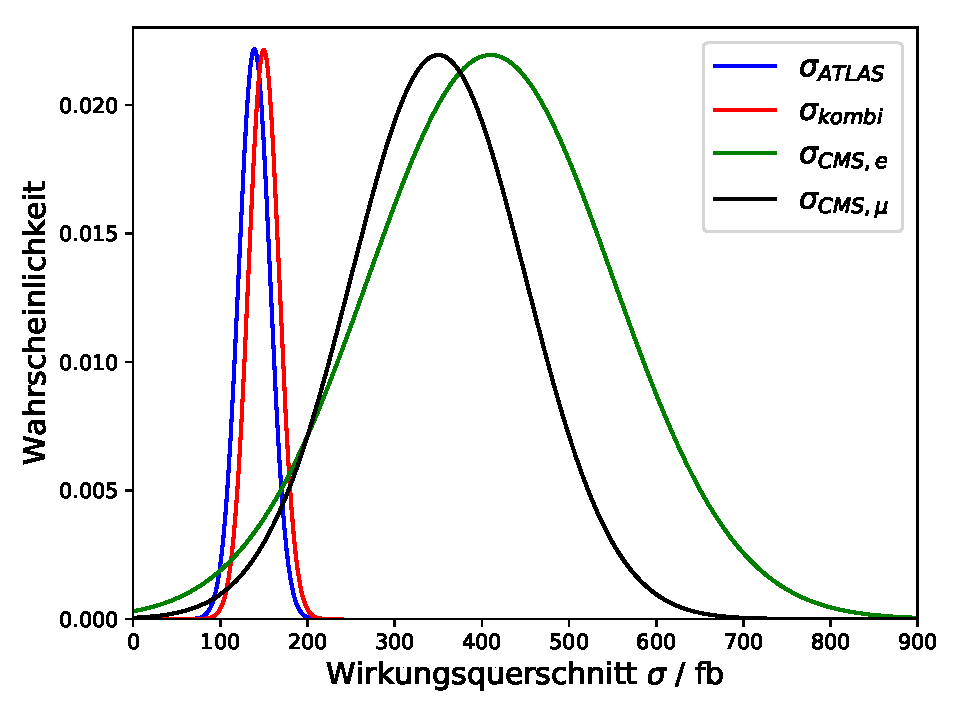
\includegraphics[width=0.5\textwidth]{Plots/gauss.pdf}
  \caption{Veranschaulichung der gaußverteilten Unsicherheiten um den Mittelwert der verschiedenen Messungen. Diese sind auf die selbe Höhe des Peaks normiert.}
  \label{fig:gau}
\end{figure}

\section{Korrelationsstudie}
Um den Einfluss möglicher Korrelationen auf die Kombination zu untersuchen, wird eine Korrelationsstudie durchgeführt. Dabei wird zunächst nur eine Korrelation zwischen den beiden CMS-Messungen untersucht. Hierfür werden die Ergebnisse aus Kapitel~\ref{phasencms} verwendet. Die verwendete Korrelationsmatrix ist symmetrisch, positiv semidefinit und hat die Form:
\begin{align}
  \text{Corr}_{\sigma,\text{CMS}}\,=\begin{pmatrix}
  1 & \rho_{e, \mu}\\
  \rho_{\mu, e} & 1
  \end{pmatrix}.
  \label{eqn:matrix1}
\end{align}
Für eine erste Betrachtung wird $\rho_{e, \mu}= \rho_{\mu, e}$ im Bereich $[-0,9;~0,9]$ mit einer Schrittweite von $0,1$ variiert. Das Ergebnis der Kombinationen der beiden Lepton+Jets-Produktionswirkungsquerschnitte von CMS unter Verwendung der Korrelationsmatrix $\text{Corr}_{\sigma,\text{CMS}}$ ist in Abbildung~\ref{fig:corrcms} dargestellt. Dabei lässt sich ein nahezu konstanter Verlauf erkennen, der lediglich im Bereich hoher positiver Korrelationen vom Fall vernachlässigter Korrelation abweicht. Da keine größeren Abweichungen zu erkennen sind, scheint die Korrelation zwischen den beiden Messungen keinen größeren Einfluss auf die Kombination zu haben.
Dies rechtfertigt die Annahme, dass die Messungen in dem genutzten Modell als unkorreliert betrachtet werden können. Die großen Fehlerbalken lassen sich auf die großen Unsicherheiten der beiden Messungen zurückführen. Zudem wachsen sie bei einer positiven Korrelation weiter an, wohingegen sie bei der negativen Korrelation geringer werden. Dies lässt sich mit dem Zusammenhang:
\begin{align}
  \sigma_{\text{Fehler, kombi}} = \sigma_{\text{Fehler, A}}^2 + 2\rho\sigma_{\text{Fehler, A}}\sigma_{\text{Fehler, B}} + \sigma_{\text{Fehler, B}}^2
\end{align}
zur Berechnung der Unsicherheiten der Kombination erklären.\\
Um zu untersuchen, ob das beobachtete Verhalten auch bei einer Kombination mit ATLAS Gültigkeit behält, wird eine Korrelationsstudie zwischen den CMS-Messungen bei der Kombination mit der ATLAS-Messung durchgeführt. Die entsprechende Korrelationsmatrix hat die Form:
\begin{align}
  \text{Corr}_{\sigma,\text{CMS}}\,=\begin{pmatrix}
  1 & 0 & 0\\
  0 & 1 &\rho_{e, \mu}\\
  0 & \rho_{\mu, e} & 1
  \end{pmatrix}.
  \label{eqn:matrix2}
\end{align}
In diesem Fall wird der Korrelationskoeffizient $\rho_{e, \mu}= \rho_{\mu, e}$ ebenfalls im Bereich $[-0,9;~0,9]$ variiert. Bei der Betrachtung von Abbildung~\ref{fig:corrca} fällt deutlich auf, dass die beiden CMS-Messungen bei einer Kombination mit dem EFT\textit{fitter} nicht stark gewichtet werden. Dies hat wieder die in Kapitel~\ref{kombi} genannte Ursache. Aus diesem Grund sind die Fehlerbalken deutlich kleiner als bei der Korrelationstudie, die ausschließlich zwischen den CMS-Produktionswirkungsquerschnitten durchgeführt wurde. Eine Abweichung wird lediglich bei sehr großen negativen Korrelationskoeffizienten beobachtet. Dies lässt sich damit erklären, dass durch die Korrelation die CMS-Messungen stärker gewichtet wird. Im restlichen Verlauf von Abbildung~\ref{fig:corrca} wird auf Grund der großen Unsicherheiten dieser Messungen die ATLAS-Messung stärker gewichtet, sodass sich auch die Kombination unter der Annahme einer Korrelation stark dem ATLAS-Messwert annähert. Für den Bereich $[-0,5;~0,9]$ zeigt sich auch in diesem Fall, dass die Korrelation bei der Kombination keinen größeren Einfluss hat, sodass die Annahme keine Korrelation zu berücksichtigen, gerechtfertigt wäre. Da jedoch im Bereich $[-0,9;~-0,6]$ eine deutliche Abweichung von dem ATLAS-Messwert vorhanden ist, sind weitere Untersuchungen zur Korrelation zwischen den CMS-Messungen sinnvoll.\\
\begin{figure}
  \centering
  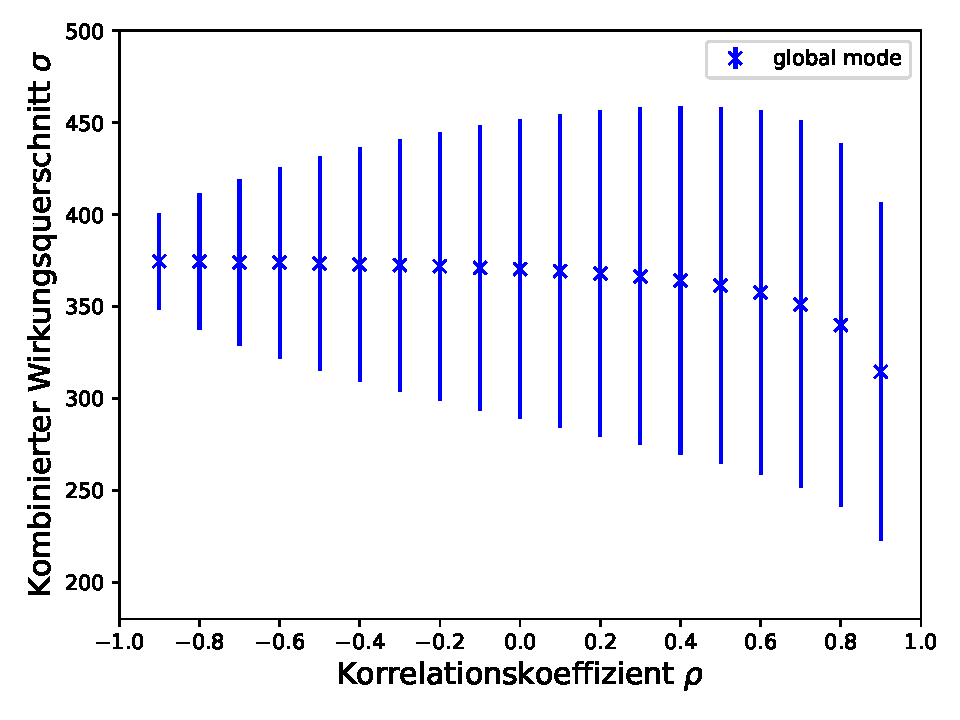
\includegraphics[width=0.5\textwidth]{Plots/corr_CMS.pdf}
  \caption{Untersuchung der Auswirkung verschiedener Korrelationen zwischen $[-0,9;~0,9]$ zwischen den beiden Lepton+Jets-Produktionswirkungsquerschnittsmessungen von CMS.}
  \label{fig:corrcms}
\end{figure}
\begin{figure}
  \centering
  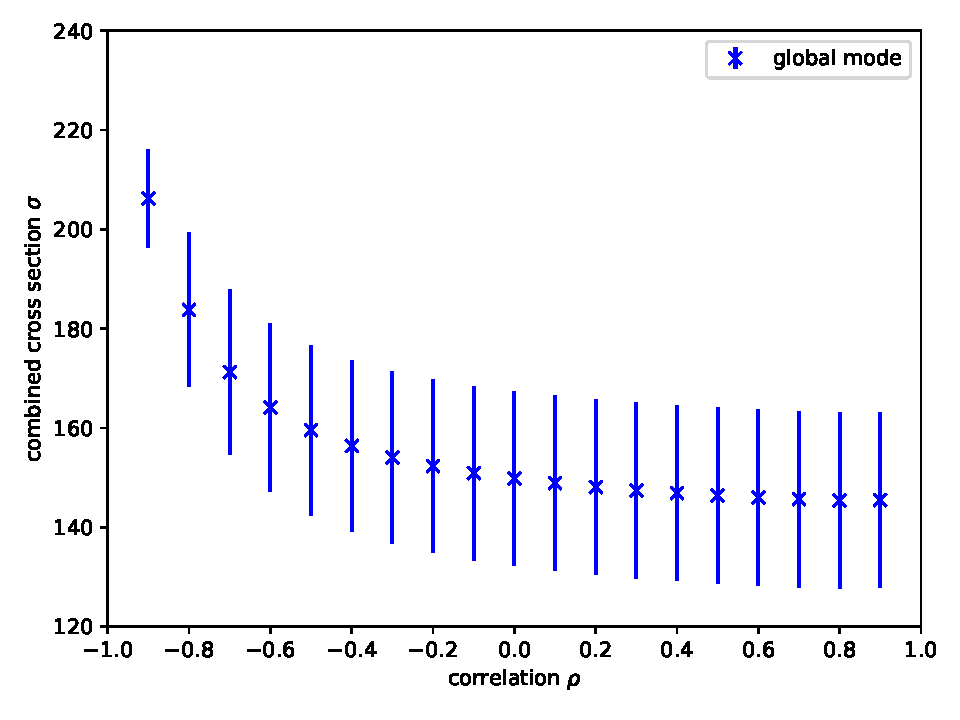
\includegraphics[width=0.5\textwidth]{Plots/fcorr_cms.pdf}
  \caption{Untersuchung der Auswirkung verschiedener Korrelationen zwischen $[-0,9;~0,9]$ zwischen den beiden Lepton+Jets-Produktionswirkungsquerschnittsmessungen von CMS, bei einer Kombination mit der Messung von ATLAS.}
  \label{fig:corrca}
\end{figure}
\begin{figure}
  \centering
  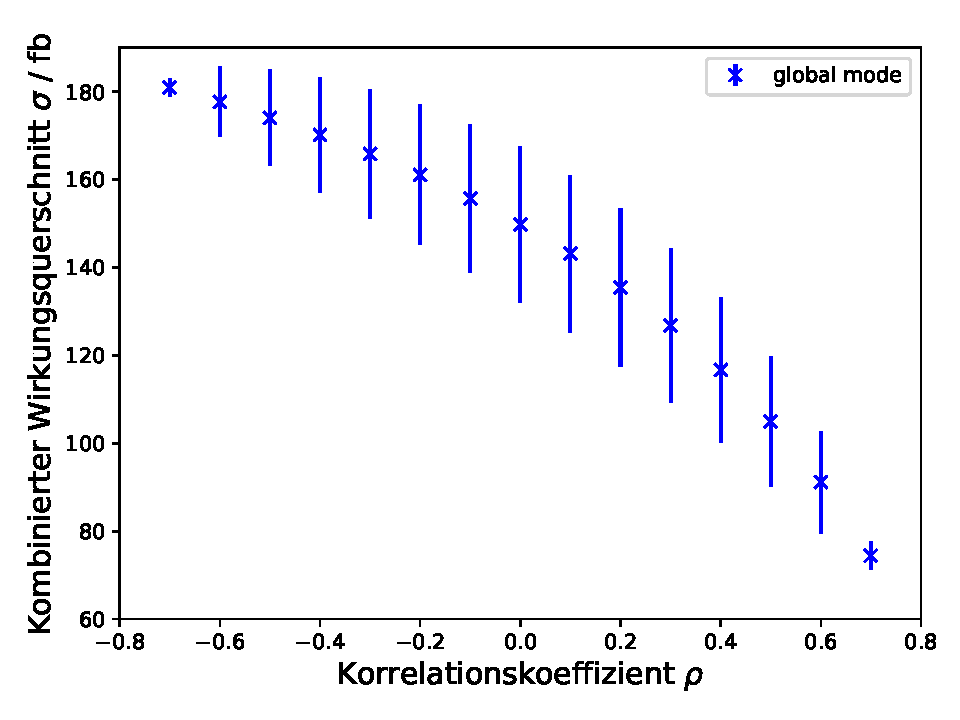
\includegraphics[width=0.5\textwidth]{Plots/corr_CA.pdf}
  \caption{Untersuchung der Auswirkung verschiedener Korrelationen zwischen $[-0,7;~0,7]$ zwischen den beiden Lepton+Jets-Produktionswirkungsquerschnittsmessungen von CMS und der ATLAS-Messung.}
  \label{fig:corrCA}
\end{figure}
Zuletzt wird die Korrelation zwischen der ATLAS-Messung und den CMS-Messungen untersucht. Die dazu verwendete Korrelationsmatrix hat die Form:
\begin{align}
  \text{Corr}_{\sigma,\text{CMS}}\,=\begin{pmatrix}
  1 & \rho_{e, \mu} & \rho_{e, \mu}\\
  \rho_{e, \mu} & 1 &0\\
  \rho_{e, \mu} & 0 & 1
  \end{pmatrix} \, .
  \label{eqn:matrix2}
\end{align}
Um die Semidefinitheit dieser Matrix zu gewährleisten, wird der Korrelationskoeffizient entsprechend einer Schrittweite von $0,1$ im Bereich $[-0,7;~0,7]$ variiert. In Abbildung~\ref{fig:corrCA} sind die sich ergebenden Ergebnisse dargestellt. Es fällt auf, dass der Verlauf stark mit $\rho_{e, \mu}$ variiert.
Dies zeigt, dass das verwendete Modell zur Kombination der Messungen sensitiv gegenüber Korrelationen zwischen den Messungen des $t\bar{t}\gamma$ Produktionswirkungsquerschnitts von ATLAS und CMS ist.
Die statistischen Unsicherheiten der beiden Messungen können nicht korreliert sein, die systematischen jedoch schon. Diese Unsicherheiten sind bei ATLAS größer als die statistischen Unsicherheiten, sodass dies zusätzlich die Untersuchung möglicher Korrelationen der Messungen motiviert. Da das verwendete Modell eine Abhängigkeit von dieser Korrelation besitzt, ist die Annahme, dass die Messungen nicht korreliert sind somit für die Kombination nicht gerechtfertigt.

\section{Interpretation der Ergebnisse}
Zusammenfassend lässt sich feststellen, dass eine einfache Kombination mit der Annahme unkorrelierter Messungen nicht sinnvoll ist. Dies liegt, neben der Erweiterung des Phasenraums der CMS-Messungen und der Extrapolation der Unsicherheiten, an der Abhängigkeit des Kombinationsergebnisses von einer Korrelation zwischen den Messungen.
Mögliche Lösungen sind genauere Rechnungen, um den Faktor $f$ zwischen den Phasenräumen nicht über eine Näherung zwischen LO- und NLO-Rechnungen zu bestimmen. Zudem sollten Messungen, die kombiniert werden sollen, möglichst im selben Phasenraum erfolgen oder nur eine geringen Unterschied besitzen.
Außerdem zeigen die Ergebnisse aus der Korrelationsstudie, dass die Annahme, dass die Messungen nicht korreliert sind, nur für die beiden CMS-Messungen gerechtfertigt ist. Für die Korrelation zwischen der ATLAS- und den CMS-Messungen bedarf es jedoch weiterer Untersuchungen.
Da unter den in dieser Arbeit getätigten Annahmen die Kombination der Messungen nahe an dem ATLAS-Wert liegt und die beiden Messungen hinsichtlich ihrer Unsicherheiten und deren Korrelationen erst weiter untersucht werden müssen, wird für die weitere Arbeit nur die ATLAS-Messung verwendet.
%
%
